%%%%%%%%%%%%%%%%%%%%%%%%%%%%%%%%%%%%%%%%%
% baposter Landscape Poster
% LaTeX Template
% Version 1.0 (11/06/13)
%
% baposter Class Created by:
% Brian Amberg (baposter@brian-amberg.de)
%
% This template has been downloaded from:
% http://www.LaTeXTemplates.com
%
% License:
% CC BY-NC-SA 3.0 (http://creativecommons.org/licenses/by-nc-sa/3.0/)
%
%%%%%%%%%%%%%%%%%%%%%%%%%%%%%%%%%%%%%%%%%

%----------------------------------------------------------------------------------------
%	PACKAGES AND OTHER DOCUMENT CONFIGURATIONS
%----------------------------------------------------------------------------------------

\documentclass[a1paper,landscape,fontscale=0.45]{baposter} % Adjust the font scale/size here

\usepackage[numbers]{natbib}         % citation style AUTHOR (YEAR), or AUTHOR [NUMBER]
%\setcitestyle{round} % round brackets for citep and citet

\usepackage{graphicx} % Required for including images
\graphicspath{{../img/}} % Directory in which figures are stored

\usepackage{amsmath} % For typesetting math
\usepackage{amssymb} % Adds new symbols to be used in math mode
\usepackage{multirow}

\usepackage{booktabs} % Top and bottom rules for tables
\usepackage{enumitem} % Used to reduce itemize/enumerate spacing
\usepackage{palatino} % Use the Palatino font
\usepackage[font=small,labelfont=bf, labelformat=empty]{caption} % Required for specifying captions to tables and figures

\usepackage{url}

\usepackage{multicol} % Required for multiple columns
\setlength{\columnsep}{2em} % Slightly increase the space between columns
\setlength{\columnseprule}{0mm} % No horizontal rule between columns

\setlist[itemize]{itemsep=2pt, topsep=3pt, parsep=0pt}
\setlist[description]{itemsep=2pt, topsep=3pt, parsep=0pt, font=\normalfont\emph, leftmargin=5ex}
\setlist[enumerate]{itemsep=2pt, topsep=3pt, parsep=0pt}
%\newcommand{\compresslist}{ % Define a command to reduce spacing within itemize/enumerate environments, this is used right after \begin{itemize} or \begin{enumerate}
%\setlength{\itemsep}{1pt}
%\setlength{\parskip}{0pt}
%\setlength{\parsep}{0pt}
%}

\usepackage{fix-cm}    

\makeatletter
\newcommand\HUGE{\@setfontsize\Huge{35}{45}}
\makeatother   

\definecolor{lightblue}{rgb}{0.145,0.6666,1} % Defines the color used for content box headers

\title{\huge Planning for Transportation Problems} % Poster title

\author{Ondrej \v{S}kopek} % Author(s)

\newcommand{\insertdepartment}{Department of Theoretical Computer Science and Mathematical Logic}
\newcommand{\institute}{Faculty of Mathematics and Physics, Charles University} % Institution(s)
\newcommand{\comment}[1]{}

\begin{document}

\begin{poster}
{
headerborder=closed, % Adds a border around the header of content boxes
colspacing=3em, % Column spacing
bgColorOne=white, % Background color for the gradient on the left side of the poster
bgColorTwo=white, % Background color for the gradient on the right side of the poster
borderColor=lightblue, % Border color
headerColorOne=lightblue, % Background color for the header in the content boxes (left side)
headerColorTwo=lightblue, % Background color for the header in the content boxes (right side)
headerFontColor=white, % Text color for the header text in the content boxes
boxColorOne=white, % Background color of the content boxes
textborder=rectangle, % Format of the border around content boxes, can be: none, bars, coils, triangles, rectangle, rounded, roundedsmall, roundedright or faded
eyecatcher=false, % Set to false for ignoring the left logo in the title and move the title left
headerheight=0.15\textheight, % Height of the header
headershape=rectangle, % Specify the rounded corner in the content box headers, can be: rectangle, small-rounded, roundedright, roundedleft or rounded
headerfont=\Large\bf\textsc, % Large, bold and sans serif font in the headers of content boxes
%textfont={\setlength{\parindent}{1.5em}}, % Uncomment for paragraph indentation
linewidth=2pt, % Width of the border lines around content boxes
boxpadding=1.3em
}
%----------------------------------------------------------------------------------------
%	TITLE SECTION 
%----------------------------------------------------------------------------------------
%
{\includegraphics[height=8em]{logo-en.pdf}} % First university/lab logo on the left
{\vspace{0.4em}\HUGE\bf\textsc{Planning for Transportation Problems}\vspace{0.3em}%
} % Poster title
{\Huge\textsc{Ondrej {\v{S}}kopek}\\\\\vspace{0.4em}%
%\LARGE\texttt{<oskopek@oskopek.com>}\\\vspace{0.4em}%
\LARGE\textsc{\insertdepartment{}}} % Author names and institution
{\includegraphics[width=36em]{logo-en.pdf}} % Second university/lab logo on the right

%----------------------------------------------------------------------------------------
%	OBJECTIVES
%----------------------------------------------------------------------------------------

\headerbox{Introduction}{name=introduction,column=0,row=0,span=1}{
\raggedright

Our goal is to design \textit{domain-specific} planners 
for several variants of the \textit{Transport} domain, introduced in the 2008 International Planning Competition (IPC).

Transport, in its basic form, consists of a road network with items located at specified locations. The items are to be delivered to their destinations
using a fleet of vehicles. Our aim is to deliver all items
with the least total cost, where the cost of individual actions is dependent on the domain variant.
}




%----------------------------------------------------------------------------------------
%	REFERENCES
%----------------------------------------------------------------------------------------

\headerbox{References}{name=references,column=0,above=bottom,span=2}{
\raggedright

\renewcommand{\section}[2]{\vskip 0.05em} % Get rid of the default "References" section title
\nocite{*} % Insert publications even if they are not cited in the poster
\scriptsize{ % Reduce the font size in this block
\vspace{-0.7em}
\setlength{\bibsep}{0pt plus 0.3ex}
\bibliographystyle{plain}
\bibliography{../../bp/en/bibliography-poster.bib} % Use sample.bib as the bibliography file
\vspace{-1em}
}}

%----------------------------------------------------------------------------------------
%	MATERIALS AND METHODS
%----------------------------------------------------------------------------------------

\headerbox{Materials \& Methods}{name=method,column=0,below=introduction,above=references}{ % This block's bottom aligns with the bottom of the conclusion block
\raggedright

The performance of our planners is compared to that of the planners taking part in the IPCs. Our planners are benchmarked using:
\begin{itemize}
\item 30 minutes of CPU time,
\item 4 GB of RAM,
\item limited to one core per planner, and
\item run on the clusters of MetaCentrum.
\end{itemize}

\textbf{Sequential planners}:

{
\setlength{\tabcolsep}{3pt} % General space between cols (6pt standard)
\renewcommand{\arraystretch}{1} % General space between rows (1 standard)
\begin{tabular}{ll}
\multirow{2}{*}{\textit{MSFA3}} & Meta-heuristically weighted SFA with\\
& the package and vehicle dist. heuristic\\[4pt]
\multirow{2}{*}{\textit{MSFA5}} & Meta-heuristically weighted SFA with\\
& the general marking heuristic\\[4pt]
\textit{RRAPN} & Rand. Restart Around Path Nearby
\end{tabular}

\vspace{0.1cm}
\textbf{Temporal planners}:
\vspace{0.05cm}

{
\setlength{\tabcolsep}{3pt} % General space between cols (6pt standard)
\renewcommand{\arraystretch}{1} % General space between rows (1 standard)
\begin{tabular}{ll}
\textit{MSFA5Sched} & Scheduled MSFA5\\[2pt]
\textit{RRAPNSched} & Scheduled RRAPN\\[2pt]
\textit{TFD2014} & Temporal Fast Downward 2014\\[2pt]
\textit{TRRAPN} & Temporal RRAPN
\end{tabular}
}
}
}

%----------------------------------------------------------------------------------------
%	Further Information
%----------------------------------------------------------------------------------------

\headerbox{Further Information}{name=further,column=3,span=1,aligned=references}{
\raggedright

Binaries and source code can be found at:
\begin{center}
\vspace{-0.5em}
\footnotesize
\url{http://github.com/oskopek/TransportEditor}
\end{center}
\vspace{-0.6em}
Contact the author at:
\begin{center}
\vspace{-0.6em}
\texttt{oskopek@oskopek.com}
\end{center}
\vspace{-1.2em}
}

%----------------------------------------------------------------------------------------
%	CONCLUSION
%----------------------------------------------------------------------------------------

\headerbox{Conclusion}{name=conclusion,column=3,span=1,row=0,above=further}{
\raggedright

The attained results show that domain-specific information can be leveraged
to generate plans of better quality.

Despite the broad misconception that they are not useful in practice,
we have not managed to beat all of them even when leveraging knowledge acquired by analyzing Transport.

There remain more approaches to try:
\begin{itemize}
\item Hierarchical Task Networks: 
HTN planning uses \textit{tasks},
a higher level, domain-specific description of sequences of operators
to carry out some goal \citep{Ghallab2004}.

\item Pointer Networks and Reinforcement Learning: 
A recent attempt at training special architectures of neural networks to solve TSP problem instances using reinforcement learning  \citep{Bello2016}.

\item Learning a domain-specific heuristic function: A
trained neural network can be used as a heuristic for state space search,
which may help when creating a heuristic is simply too challenging \citep{Chen2011}.
\end{itemize}

To make problem analysis and planner design easier, we have developed TransportEditor \citep{Skopek2017}.
\begin{center}
\vspace{-0.5em}
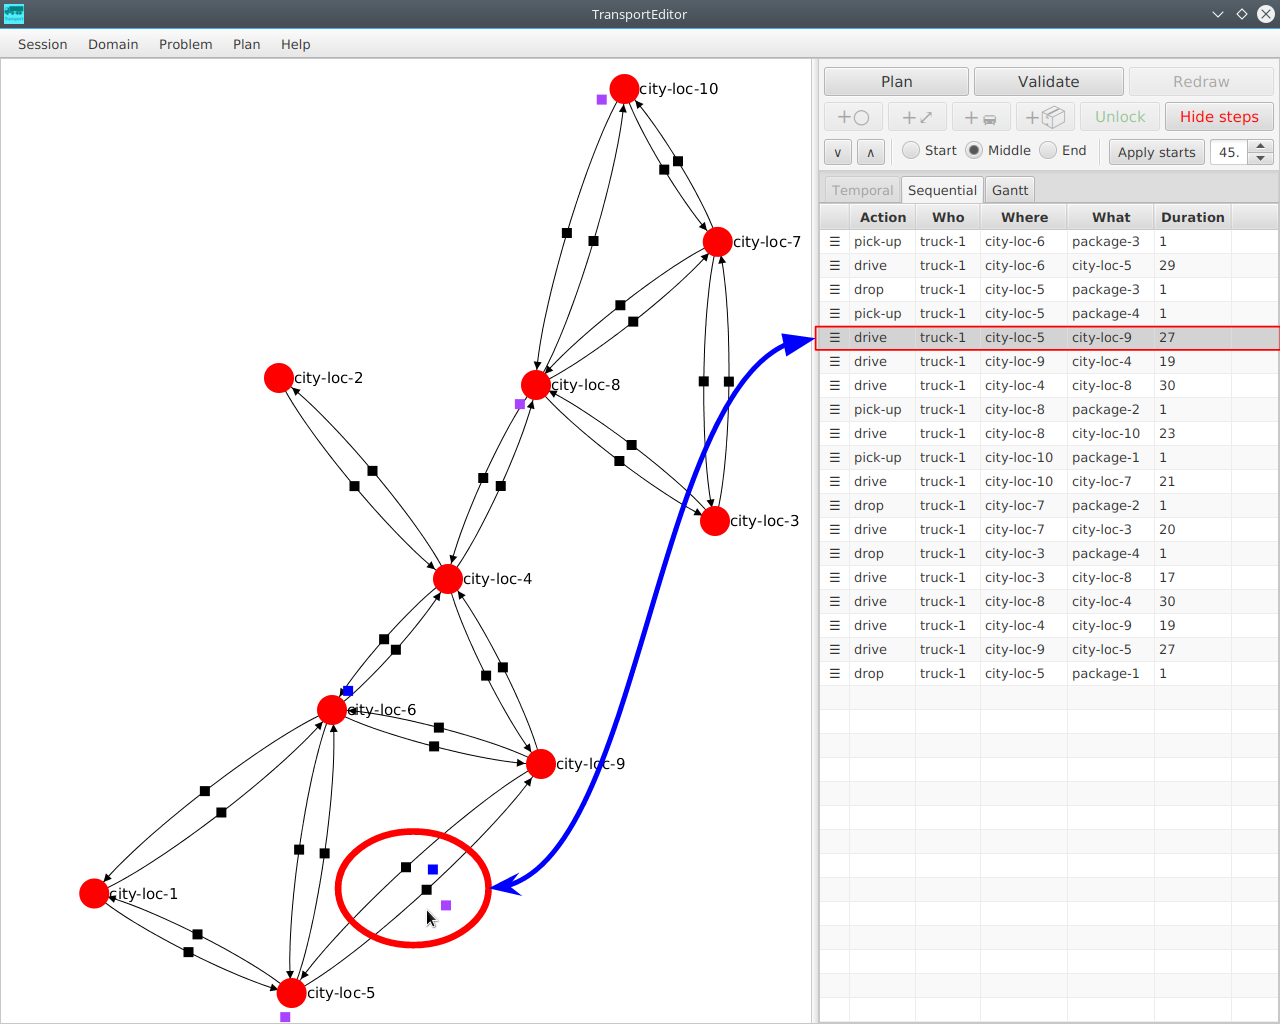
\includegraphics[width=\linewidth{},height=13em]{../../bp/img/transporteditor_planstates.png}
\captionof{figure}{\textbf{Figure 5:} Tracing a plan in TransportEditor.}
\end{center} 

}

%----------------------------------------------------------------------------------------
%	Acknowledgements
%----------------------------------------------------------------------------------------

\headerbox{Acknowledgements}{name=ack,column=2,span=1,aligned=references}{
\raggedright

Thank you to prof.\;RNDr.\;Roman\;Bart{\'{a}}k, Ph.D., my advisor.

Provided access to the computing facilities of MetaCentrum is greatly appreciated.
}





%----------------------------------------------------------------------------------------
%	RESULTS
%----------------------------------------------------------------------------------------

\headerbox{Results}{name=results,column=1,row=0,span=2,above=references}{
\raggedright

\vspace{-0.4em}
\begin{multicols}{2}
We have designed and implemented Transport planners that are able to beat
all results from the sequential
and temporal satisficing tracks of the 2008 (Figure~1 and 2) and 2011 IPCs (Figure 3).

In the 2014 IPC (Figure 4), we would have attained second place on overall quality in the Transport domain, behind the impressive result of Mercury.

Across datasets, the performance of our planners is
satisfactory, compared to domain-independent planners
participating in the original IPCs. This can be observed in Table~1 and 2.

Performance of domain-independent planners is generally very impressive, given the difficulty of the problem they are solving.
Our figures only show the three best domain-independent planners on
the given dataset.

\begin{center}
\begin{tabular}{lr}
\toprule
\textbf{Planner} & \textbf{Avg.\;quality}\\
\midrule
MSFA3 & 0.923\\
MSFA5 & \textbf{0.924}\\
RRAPN & 0.894\\
\bottomrule
\end{tabular}
\captionof{table}{\textbf{Table 1:} Average quality on sequential datasets.}

\vspace{0.7cm}
\begin{tabular}{lr}
\toprule
\textbf{Planner} & \textbf{Avg.\;quality}\\
\midrule
MSFA5Sched & 0.483\\
RRAPNSched & 0.905\\
TRRAPN & \textbf{0.934}\\
\bottomrule
\end{tabular}
\captionof{table}{\textbf{Table 2:} Average quality on the temporal dataset.}
\end{center}

\comment{
\textbf{IPC 2008 --- Sequential satisficing} (Figure~1)

\vspace{0.15cm}
Our best planner on the this dataset, RRAPN:
\begin{itemize}
\item RRAPN achieves the best total quality of \textbf{27.85}/30;
\item MSFA3 and MSFA5 obtain better results than RRAPN on smaller problems
(2--3, 21--22), and are able to generate very good results even on larger problems (14--20, 28--29).
\end{itemize}
MSFA5 marginally comes out on top as the better one of the two MSFA planners on total quality. All three of our planners beat all planners from the original competition.

\vspace{0.15cm}
\textbf{IPC 2008 --- Temporal satisficing} (Figure~2)
\vspace{0.15cm}

We improved over recent domain-independent temporal planners (TFD2014):
\begin{itemize}
\item MSFA5Sched achieves a total of 14.50/30;
\item RRAPNSched achieves 27.16/30; and
\item TRRAPN beats both with 28.02/30.
\end{itemize}
MSFA5 does not generate plans of much variety,
hence produces worse scheduled plans.

TRRAPN performs
better on
large problems (10, 19, or 30), where RRAPNSched cannot plan well with fuel,
and worse on smaller ones (4--7).

\vspace{0.15cm}
\textbf{IPC 2011 --- Sequential satisficing} (Figure~3)
\vspace{0.15cm}

All our planners beat all competition planners:
\begin{itemize}
\item RRAPN even achieves better scores than all original planners on all individual problems, with a total of 18.81/20; and
\item MSFA planners' performance
is almost indistinguishable, even on single problems. In total, MSFA3 achieves 18.78 and MSFA5 achieves 18.75.
\end{itemize}
MSFA planner results are complementary to RRAPN on some problems (3--6, 10--12, 13--15).


\vspace{0.15cm}
\textbf{IPC 2014 --- Sequential satisficing} (Figure~4)
\vspace{0.15cm}

The winner on Transport was the Mercury planner, achieving
a stunning 20/20 total quality. The runner-up, yahsp3-mt, achieved a score of only 10.74/20
and all other planners achieved sub 10/20 total quality.

After adding the results of our planners:
\begin{itemize}
\item RRAPN manages to outperform yahsp3-mt with 15.91/20, yet it fails
to match the results of Mercury.
\item Both MSFA planners outperform RRAPN with qualities just under 18.50/20.

The results of MSFA3 and MSFA5 on this dataset are almost identical.
\end{itemize}
None of our planners came reasonably close to beating Mercury (at 19.25/20).
However, they do marginally outperform it on problems 4--7, 9--10, 12, and 18--19.
}
\end{multicols}

\vspace{0.2em}
\begin{multicols}{2}
\begin{center}
\includegraphics[width=\linewidth]{seq-sat-6-quality.pdf}
\captionof{figure}{\textbf{Figure 1:} IPC 2008 --- Sequential satisficing}
\includegraphics[width=\linewidth]{seq-sat-7-quality.pdf}
\captionof{figure}{\textbf{Figure 3:} IPC 2011 --- Sequential satisficing}
\end{center}
\begin{center}
\includegraphics[width=\linewidth]{tempo-sat-6-quality.pdf}
\captionof{figure}{\textbf{Figure 2:} IPC 2008 --- Temporal satisficing}
\includegraphics[width=\linewidth]{seq-sat-8-quality.pdf}
\captionof{figure}{\textbf{Figure 4:} IPC 2014 --- Sequential satisficing}
\end{center}
\end{multicols}
}




%----------------------------------------------------------------------------------------

\end{poster}

\end{document}
